\chapter{Previous Year Questions}

\section*{Introduction to Artificial Intelligence [CO1]}

\subsection*{Artificial Intelligence}

\begin{Question}[4][CO1 \rgbGray{/} S-24]
Explain an Al Expert System with its three basic building blocks and necessary diagram.
\end{Question}

\begin{Question}[4][CO1 \rgbGray{/} S-23]
   Explain the difference between artificial intelligence (AI), machine learning (ML) and deep learning (DL). Draw the hierarchical tree structure of Al mentioning all the sub-fields of Al.
\end{Question}

\vspace{1em}
\begin{Question}[4][F-22 \rgbGray{/} S-22]
   Differentiate between machine learning (ML) and deep learning (DL) in your own words.

   Differentiate between supervised learning and un-supervised / re-enforcement learning.
\end{Question}

\vspace{1em}
\begin{Question}[4][S-21 \rgbGray{/} F-23]
   What is Turing Test? What are the capabilities that an intelligent machine should possess to pass the Turing Test? What are the additional capabilities to pass the Total Turing Test?
\end{Question}



\subsection*{Intelligent AI Agent}

\begin{Question}[2][F-22]
   What is rational agent in artificial intelligence? State the characteristics that a rational agent should possess.
\end{Question}

\begin{Question}[4][S-21]
   Differentiate the following agents in your own words: Simple Reflex Agent and Model-based Reflex Agent.

   Explain the components of the intelligent agent in your own words.
\end{Question}

\vspace{1em}
\begin{Question}[4][CO1 \rgbGray{/} S-24]
   Suppose you are developing an Al-powered Drone (Al Agent) for monitoring the overall environment of UAP. Note that the agent should notify the UAP administration whenever any illegal/violent activities are being observed. Specify the \textbf{PEAS} for the agent \textbf{UAP Environment Monitoring Agent}
\end{Question}

\vspace{1em}
\begin{Question}[4][F-22 \rgbGray{/} S-21]
   Suppose, you are developing a \textbf{Trash Picking Robot} to clean the UAP CSE Void Space. Specify the PEAS description of your intelligent agent.
\end{Question}
\begin{Question}[4]
   For the above agent, characterize the environment whether it is:
   $(i)$ fully observable or partially observable, \\
   $(ii)$ deterministic or stochastic,
   $(iii)$ episodic or sequential,
   $(iv)$ single agent or multi-agent.
   
   Explain your answer with your own logic.
\end{Question}

\vspace{1em}
\begin{Question}[4][F-23]
   To produce good quality strawberry jelly, it is important to segregate the ripe strawberries and use them for production. Using bad-quality or unripe strawberries, can lower the quality of the jelly. Now, classifying the strawberries can be done manually, but it would be tedious for humans as a factory might process thousands of strawberries daily. Hence, we can incorporate an Al agent to help us. Specify the PEAS description of a \textbf{Strawberry Classification Agent}.
\end{Question}

\vspace{1em}
\begin{Question}[4][CO1 \rgbGray{/} S-23]
   Suppose two intelligent agents playing \textbf{GO board game} where one of them is called \textbf{AlphaGo} (Al agent), and the other is called \textbf{Lee Sedol} (human being), Specify the \textbf{PEAS} for the agent "AlphaGo".
\end{Question}


\vspace{2em}
\section*{Searching Algorithms [CO2]}

\subsection*{Uniformed Searching Algorithms}

\begin{Question}[4]
   Generate a state space graph of 7 nodes. Determine the sequences/orders in which the nodes of a search tree will be visited for: \ 
   $(i)$ Iterative Deepening Search (IDS)
   $(ii)$ Uniform Cost Search (UCS)
\end{Question}

\vspace{1em}
\begin{Question}[6]
   Generate a state space graph of 6 nodes. Show the differences between the sequences/orders in which the nodes of a search tree will be visited for: \
   $(i)$ Breadth-First Search (BFS) \ 
   $(ii)$ Depth-First Search (DFS) and \\
   $(iii)$ Iterative Deepening Search (IDS)
\end{Question}



\subsection*{A* Search Algorithm}

\begin{Question}[7][CO2 \rgbGray{/} S-24]
   Suppose, your target is to reach the goal node $G$ from start node $S$ with the optimum cost. Simulate the following problem with \textbf{A* search algorithm} and show the shortest path with the fringe for each iteration. Assume that states with earlier alphabetical order are expanded first. Consider the heuristics as follows. You have to draw the Search Tree.

   \vspace{1em}
   \begin{center}
      \begin{minipage}{0.4\textwidth}
         \begin{tabular}{l}
            $h(S) =$ \ (Last 2 digits of id \% 2) + 1 \\
            $h(A) =$ \ (Last 2 digits of id \% 3) + 2 \\
            $h(B) =$ \ (Last 2 digits of id \% 4) + 3 \\
            $h(C) =$ \ $h(B)$ + 2
         \end{tabular}
      \end{minipage}%
      \begin{minipage}{0.45\textwidth}
         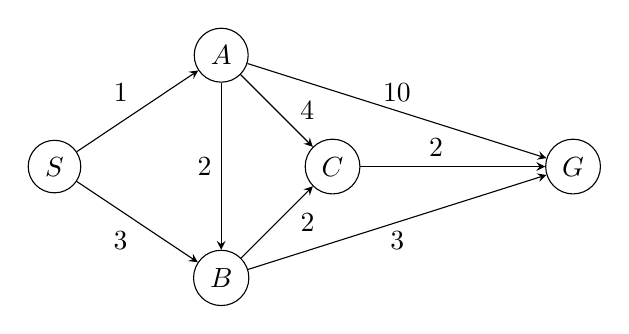
\begin{tikzpicture}
            [node distance=2cm, main node/.style={circle,draw,minimum size=6mm}]
            \node[main node] (s) {$S$};
            \node[main node, above right of=s, xshift=2em] (a) {$A$};
            \node[main node, below right of=s, xshift=2em] (b) {$B$};
            \node[main node, below right of=a] (c) {$C$};
            \node[main node, right of=c, xshift=3em] (g) {$G$};

            \draw[-stealth] (s) -- node[above left] {1} (a);
            \draw[-stealth] (s) -- node[below left] {3} (b);
            \draw[-stealth] (a) -- node[left] {2} (b);
            \draw[-stealth] (a) -- node[right=0.5em] {4} (c);
            \draw[-stealth] (a) -- node[above] {10} (g);

            \draw[-stealth] (b) -- node[right=0.5em] {2} (c);
            \draw[-stealth] (b) -- node[below] {3} (g);
            \draw[-stealth] (c) -- node[above left] {2} (g);
         \end{tikzpicture}
      \end{minipage}
   \end{center}
\end{Question}

\vspace{2em}
\begin{Question}[7][CO2 \rgbGray{/} F-22\\F-21\\S-21]
   Suppose, your target is to reach the goal node $G$ from the start node $S$ with the optimal cost. Simulate the following problem with \textbf{A* Search algorithm} and determine the shortest path with fringe for each iteration. Consider the heuristic values of the nodes as follows:

   \vspace{1em}
   \begin{center}
      \begin{minipage}{0.4\textwidth}
         \begin{tabular}{l}
            $h(S) =$ \ 1 \\
            $h(A) =$ \ $h(S)$ + 2 \\
            $h(B) =$ \ $h(A)$ + 3 \\
            $h(C) =$ \ $h(B)$ + 4 \\
            $h(G) =$ \ 0
         \end{tabular}
      \end{minipage}%
      \begin{minipage}{0.4\textwidth}
         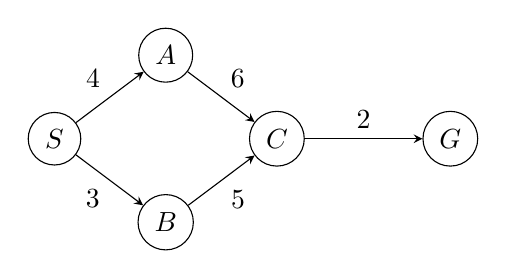
\begin{tikzpicture}
            [node distance=1.5cm, main node/.style={circle,draw,minimum size=6mm}]
            \node[main node] (s) at (0,0) {$S$};
            \node[main node, above right of=s, xshift=1em] (a) {$A$};
            \node[main node, below right of=s, xshift=1em] (b) {$B$};
            \node[main node, below right of=a, xshift=1em] (c) {$C$};
            \node[main node, right of=c, xshift=2em] (g) {$G$};

            \draw[-stealth] (s) -- node[above left] {4} (a);
            \draw[-stealth] (s) -- node[below left] {3} (b);
            
            \draw[-stealth] (a) -- node[above right] {6} (c);
            \draw[-stealth] (b) -- node[below right] {5} (c);
            
            \draw[-stealth] (c) -- node[above] {2} (g);
         \end{tikzpicture}
      \end{minipage}
   \end{center}
\end{Question}

\vspace{2em}
\begin{Question}[7][CO2 \rgbGray{/} S-23]
Suppose, your target is to reach the goal node $G$ from start node $S$ with the most optimum cost. Simulate the following graph problem with \textbf{A* search algorithm}, draw the search tree and determine the optimal path with fringe for each iteration. Assume that states with earlier alphabetical order are expanded first if two nodes have the same evaluation values. The heuristic values, $h(n)$ of the 6 nodes and the path costs, $g(n)$ are given below.

\vspace{1em}
\begin{center}
   \begin{minipage}{0.4\textwidth}
      \begin{tabular}{l}
         $h(S) =$ \ (Last 2 digits of id) \% 3 + 5 \\
         $h(A) =$ \ (Last 2 digits of id) \% 2 + 4 \\
         $h(B) =$ \ (Last 2 digits of id) \% 4 + 3 \\
         $h(C) =$ \ $h(A)$ + 2 \\
         $h(D) =$ \ $h(B)$ + 3
      \end{tabular}
   \end{minipage}%
   \begin{minipage}{0.4\textwidth}
      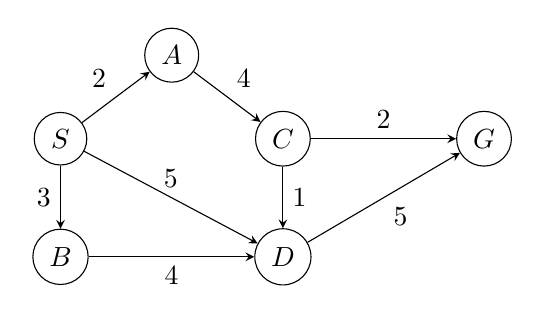
\begin{tikzpicture}
         [node distance=1.5cm, main node/.style={circle,draw,minimum size=6mm,}]
         \node[main node] (a) at (0,0) {$A$};
         \node[main node, below left of=a, xshift=-1em] (s) {$S$};
         \node[main node, below right of=a, xshift=1em] (c) {$C$};
         \node[main node, below of=s] (b) {$B$};
         \node[main node, below of=c] (d) {$D$};
         \node[main node, right of=c, xshift=3em] (g) {$G$};
         
         \draw[-stealth] (s) -- node[above left] {2} (a);
         \draw[-stealth] (s) -- node[left] {3} (b);
         \draw[-stealth] (s) -- node[above] {5} (d);
         
         \draw[-stealth] (a) -- node[above right] {4} (c);
         \draw[-stealth] (b) -- node[below] {4} (d);
         \draw[-stealth] (c) -- node[right] {1} (d);
         
         \draw[-stealth] (c) -- node[above] {2} (g);
         \draw[-stealth] (d) -- node[below right] {5} (g);
      \end{tikzpicture}
   \end{minipage}
\end{center}
\end{Question}

\vspace{2em}
\begin{Question}[7][CO2 \rgbGray{/} S-23\\S-22]
Suppose, your target is to reach the goal node $G$ from initial node $A$ with the optimal cost. Simulate the following problem with \textbf{A* search algorithm}. Draw the search tree and determine the shortest path with fringe for each iteration. Assume that the states with earlier alphabetical order are to be expanded first. The heuristic values of the 6 nodes are as follows:

\vspace{2em}
\begin{center}
   \begin{minipage}{0.4\textwidth}
      \begin{tabular}{l}
         $h(S) =$ \ (Last 2 digits of id) \% 4 + 2 \\
         $h(A) =$ \ (Last 2 digits of id) \% 5 + 3 \\
         $h(B) =$ \ (Last 2 digits of id) \% 6 + 1 \\
         $h(C) =$ \ (Last 2 digits of id) \% 5 + 2 \\
         $h(D) =$ \ (Last 2 digits of id) \% 4 + 1
      \end{tabular}
   \end{minipage}%
   \begin{minipage}{0.4\textwidth}
      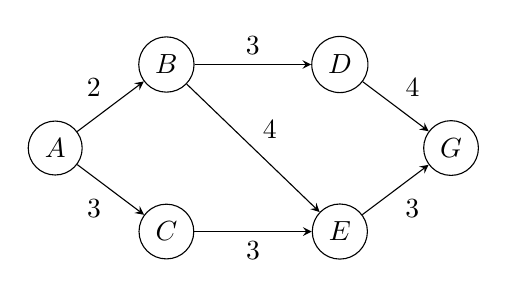
\begin{tikzpicture}
         [node distance=1.5cm, main node/.style={circle,draw,minimum size=6mm,}]
         \node[main node] (a) at (0,0) {$A$};
         \node[main node, above right of=a, xshift=1em] (b) {$B$};
         \node[main node, below right of=a, xshift=1em] (c) {$C$};
         \node[main node, right of=b, xshift=2em] (d) {$D$};
         \node[main node, right of=c, xshift=2em] (e) {$E$};
         \node[main node, below right of=d, xshift=1em] (g) {$G$};

         
         \draw[-stealth] (a) -- node[above left] {2} (b);
         \draw[-stealth] (a) -- node[below left] {3} (c);
         
         \draw[-stealth] (b) -- node[above] {3} (d);
         \draw[-stealth] (b) -- node[above right] {4} (e);
         \draw[-stealth] (c) -- node[below] {3} (e);
         
         \draw[-stealth] (d) -- node[above right] {4} (g);
         \draw[-stealth] (e) -- node[below right] {3} (g);
      \end{tikzpicture}
   \end{minipage}
\end{center}
\end{Question}

\vspace{2em}
\begin{Question}[7][CO2 \rgbGray{/} F-23]
   Suppose, your target is to reach the goal node 'G' from start node 'S' with tho optimum cost. Simulate the following problem with \textbf{A* search algorithm} and show the shortest path with the fringe for each iteration. Assume that states with earlier alphabetical order are expanded first. There are 6 nodes in the graph where the heuristics values of the 5 nodes are as follows. Here \% refers to mod operation. You have to draw the Search Tree.

\vspace{1em}
\begin{center}
   \begin{minipage}{0.4\textwidth}
      \begin{tabular}{l}
         $h(S) =$ \ (Last 2 digits of id) \% 3 + 1 \\
         $h(A) =$ \ (Last 2 digits of id) \% 2 + 2 \\
         $h(B) =$ \ $h(S)$ + 1 \\
         $h(C) =$ \ $h(B)$ + 3 \\
         $h(D) =$ \ $h(A)$ + 2 \\
      \end{tabular}
   \end{minipage}%
   \begin{minipage}{0.4\textwidth}
      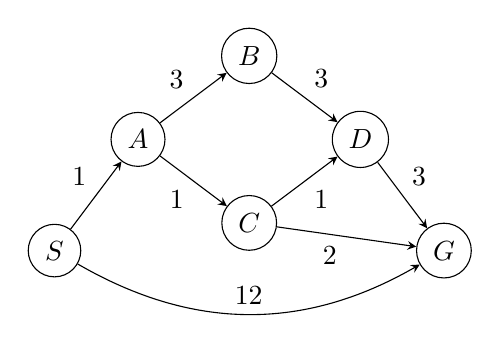
\begin{tikzpicture}
         [node distance=1.5cm, main node/.style={circle,draw,minimum size=6mm,}]
         \node[main node] (s) at (0,0) {$S$};
         \node[main node, above right of=s, yshift=1em] (a) {$A$};
         \node[main node, above right of=a, xshift=1em] (b) {$B$};
         \node[main node, below right of=a, xshift=1em] (c) {$C$};
         \node[main node, below right of=b, xshift=1em] (d) {$D$};
         \node[main node, below right of=d, yshift=-1em] (g) {$G$};

         
         \draw[-stealth] (s) -- node[above left] {1} (a);
         \draw[-stealth, bend right=30] (s) to node[above] {12} (g);
         \draw[-stealth] (a) -- node[above left] {3} (b);
         \draw[-stealth] (a) -- node[below left] {1} (c);
         \draw[-stealth] (b) -- node[above right] {3} (d);
         \draw[-stealth] (c) -- node[below right] {1} (d);
         \draw[-stealth] (c) -- node[below left] {2} (g);
         \draw[-stealth] (d) -- node[above right] {3} (g);
      \end{tikzpicture}
   \end{minipage}
\end{center}
\end{Question}

\subsection*{Admissible \& Consistent Heuristic}

\begin{Question}[5][CO2 \rgbGray{/} S-24\\F-23]
Consider the following state space graph where $A$ is the start state and $G$ is the goal state. Suppose, you are analyzing the heuristic function  $h_1$ as shown below. All the values are fixed except $h_1(C)$.

\vspace{1em}
\begin{center}
\begin{minipage}[c]{0.5\textwidth}
   \centering
   \begin{tikzpicture}[main node/.style={circle,draw,minimum size=6mm,}]
      \node[main node] (a) at (0,0) {A};
      \node[main node] (b) [above right=of a, xshift=1em] {$B$};
      \node[main node] (c) [below right=of a, xshift=1em] {$C$};
      \node[main node] (d) [below right=of b, xshift=1em] {$D$};
      \node[main node] (e) [above right=of d, xshift=1em] {$E$};
      \node[main node] (f) [below right=of d, xshift=1em] {$F$};
      \node[main node] (g) [below right=of e, xshift=1em] {$G$};
   
      \draw (a) -- node[above left] {2} (b);
      \draw (a) -- node[below left] {5} (c);
      \draw (b) -- node[left] {2} (c);

      \draw (b) -- node[above right] {6} (d);
      \draw (c) -- node[below right] {4} (d);

      \draw (d) -- node[above] {10} (g);
      \draw (d) -- node[above left] {9} (e);
      \draw (d) -- node[below left] {4} (f);

      \draw (e) -- node[above right] {2} (g);
      \draw (f) -- node[below right] {6} (g);
   \end{tikzpicture}
\end{minipage}%
\hfill
\begin{minipage}[c]{0.4\textwidth}
   \centering
   \begin{tabular}{|c|c|c|c|c|c|c|c|}\hline
      Node & A & B & C & D & E & F & G \\\hline
      $h_1$ & 9 & 7 & ? & 5 & 3 & 4 & 0 \\\hline
   \end{tabular}
\end{minipage}
\end{center}

\vspace{1em}
   $(i)$ Determine which value of $h_1(C)$ makes $h_1$ admissible?
   \qquad
   $(ii)$ Determine which value of $h_1(C)$ makes $h_1$ consistent?
\end{Question}

\vspace{1em}
\begin{Question}[5][CO2 \rgbGray{/} F-22\\S-21]
Consider the following state space graph where $A$ is the start state and $G$ is the goal state. Suppose, you are analyzing the heuristic function  $h_1$ as shown below. All the values are fixed except $h_1(B)$.

\vspace{1em}
\begin{center}
\begin{minipage}[c]{0.5\textwidth}
   \centering
   \begin{tikzpicture}[main node/.style={circle,draw,minimum size=6mm,}]
      \node[main node] (a) at (0,0) {A};
      \node[main node] (b) [above right=of a, xshift=1em] {$B$};
      \node[main node] (c) [below right=of a, xshift=1em] {$C$};
      \node[main node] (d) [below right=of b, xshift=1em] {$D$};
      \node[main node] (e) [above right=of d, xshift=1em] {$E$};
      \node[main node] (f) [below right=of d, xshift=1em] {$F$};
      \node[main node] (g) [below right=of e, xshift=1em] {$G$};
   
      \draw (a) -- node[above left] {2} (b);
      \draw (a) -- node[above] {3} (d);
      \draw (a) -- node[below left] {1} (c);

      \draw (b) -- node[above right] {4} (d);
      \draw (c) -- node[below right] {2} (d);
      
      \draw (d) -- node[above left] {3} (e);
      \draw (d) -- node[below left] {2} (f);

      \draw (e) -- node[left] {5} (f);
      \draw (e) -- node[above right] {4} (g);
      
      \draw (f) -- node[below right] {3} (g);
   \end{tikzpicture}
\end{minipage}%
\hfill
\begin{minipage}[c]{0.4\textwidth}
   \centering
   \begin{tabular}{|c|c|c|c|c|c|c|c|}\hline
      Node & A & B & C & D & E & F & G \\\hline
      $h_1$ & 8 & ? & 6 & 5 & 3 & 3 & 0 \\\hline
   \end{tabular}
\end{minipage}
\end{center}

\vspace{1em}
   $(i)$ Determine which value of $h_1(B)$ makes $h_1$ admissible?
   \qquad
   $(ii)$ Determine which value of $h_1(B)$ makes $h_1$ consistent?
\end{Question}
   
\vspace{2em}
\begin{Question}[3][CO2 \rgbGray{/} S-23\\F-21]
   Is the solution of the following 8-puzzle game has admissible heuristic? Why? Here, consider $h_1$ as number of misplaced tiles and $h_2$ as total Manhattan distance (city block distance).

   \vspace{2em}
   \begin{center}
      \begin{minipage}{4cm}
         \centering
         \begin{tabular}{l}
            \ding{242} \ $h_1(S) = ?$ \\
            \ding{242} \ $h_2(S) = ?$
         \end{tabular}
      \end{minipage}%
      \begin{minipage}{4cm}
         \begin{tabular}{|c|c|c|}\hline
            2 & 8 & 3 \\\hline
            1 & 6 & 4 \\\hline
            7 & & 5 \\\hline
            \multicolumn{3}{c}{Initial State}
         \end{tabular}
      \end{minipage}%
      \begin{minipage}{4cm}
         \begin{tabular}{|c|c|c|}\hline
            1 & 2 & 3 \\\hline
            8 & & 4 \\\hline
            7 & 6 & 5 \\\hline
            \multicolumn{3}{c}{Final State}
         \end{tabular}
      \end{minipage}
   \end{center}
\end{Question}

\vspace{2em}
\begin{Question}[3][CO2 \rgbGray{/} F-22]
   Is the solution of the following 8-puzzle game has admissible heuristic? Why? Here, consider $h_1$ as number of misplaced tiles and $h_2$ as total Manhattan distance (city block distance).

   \vspace{2em}
   \begin{center}
      \begin{minipage}{4cm}
         \centering
         \begin{tabular}{l}
            \ding{242} \ $h_1(S) = ?$ \\
            \ding{242} \ $h_2(S) = ?$
         \end{tabular}
      \end{minipage}%
      \begin{minipage}{4cm}
         \begin{tabular}{|c|c|c|}\hline
            7 & 2 & 4 \\\hline
            5 & & 6 \\\hline
            8 & 3 & 1 \\\hline
            \multicolumn{3}{c}{Initial State}
         \end{tabular}
      \end{minipage}%
      \begin{minipage}{4cm}
         \begin{tabular}{|c|c|c|}\hline
            & 1 & 2 \\\hline
            3 & 4 & 5 \\\hline
            6 & 7 & 8 \\\hline
            \multicolumn{3}{c}{Final State}
         \end{tabular}
      \end{minipage}
   \end{center}
\end{Question}